\documentclass[tikz,border=3.14mm]{standalone}
\usetikzlibrary{matrix}
\begin{document}
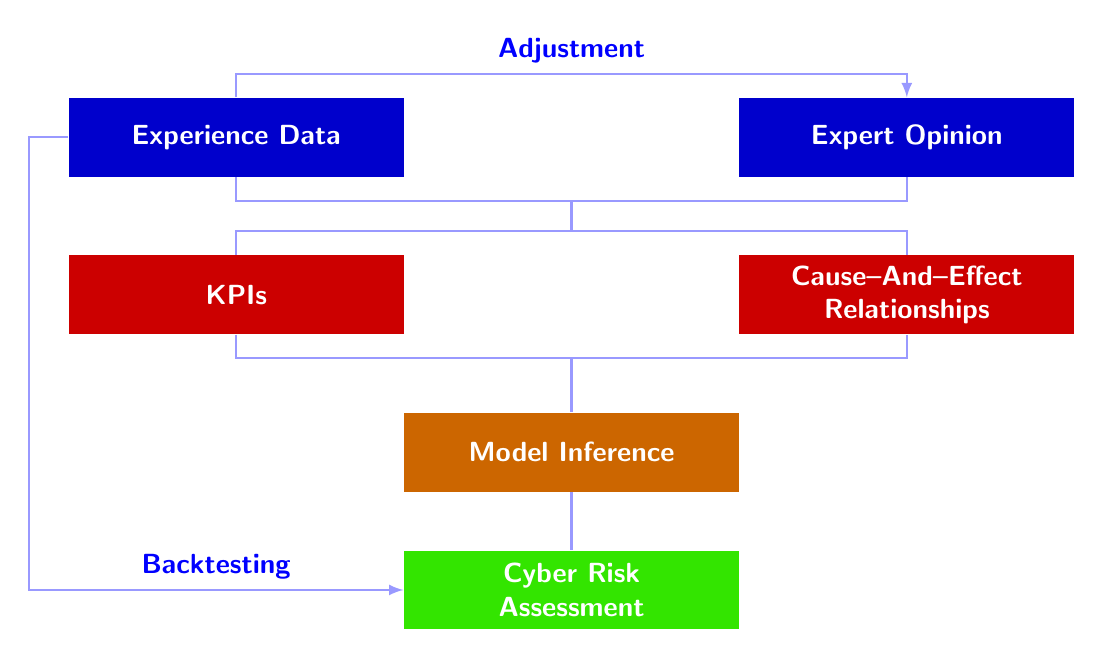
\begin{tikzpicture}[node font=\sffamily\bfseries]
\matrix[column sep=0pt,matrix of nodes,
nodes={text=white,text width=4cm,anchor=center,minimum
height=1cm,align=center}] (mat)
{
|[fill=blue!80!black]| Experience Data & & |[fill=blue!80!black]| Expert Opinion\\[1cm]
|[fill=red!80!black]| KPIs & & |[fill=red!80!black]| {Cause--And--Effect\\ Relationships}\\[1cm]
& |[fill=orange!80!black]| Model Inference & \\[0.75cm]
& |[fill=green!80!orange]| {Cyber Risk\\ Assessment} & \\
};
\begin{scope}[blue!40,thick,>=latex]
\draw[->] (mat-1-1.north) -- ++ (0,0.3) -| (mat-1-3)
node[pos=0.25,above,blue]{Adjustment};
\draw[->] (mat-1-1.west) -- ++ (-0.5,0) |- (mat-4-2)
node[pos=0.75,above,blue]{Backtesting};
\draw (mat-1-1.south) -- ++ (0,-0.3) -| (mat-1-3) coordinate[pos=0.25] (aux1)
 (mat-2-1.north) -- ++ (0,0.3) -| (mat-2-3) coordinate[pos=0.25] (aux2)
 (mat-2-1.south) -- ++ (0,-0.3) -| (mat-2-3) coordinate[pos=0.25] (aux3)
 (aux1) -- (aux2) (aux3) -- (mat-3-2) (mat-3-2) -- (mat-4-2);
\end{scope}
\end{tikzpicture}
\end{document}